\documentclass[conference]{IEEEtran}
\IEEEoverridecommandlockouts

% ---------------------------------------------------------------------------
% PACKAGES & CONFIGURATION
% ---------------------------------------------------------------------------
\usepackage{cite}
\usepackage{amsmath,amssymb,amsfonts}
\usepackage{algorithmic}
\usepackage{algorithm}
\usepackage{graphicx}
\usepackage{textcomp}
\usepackage{xcolor}
\usepackage{booktabs}
\usepackage{listings}
\usepackage{url}
\usepackage{microtype}
\usepackage{balance}

% Use hidelinks to completely REMOVE all green/colored boxes around citations and URLs
\usepackage[hidelinks]{hyperref}

\def\BibTeX{{\rm B\kern-.05em{\sc i\kern-.025em b}\kern-.08em
    T\kern-.1667em\lower.7ex\hbox{E}\kern-.125emX}}

\begin{document}

\title{AutoSecAudit: An Extensible Multi-Scanner Orchestration Engine with Automated Compliance Mapping and Delta Auditing for DevSecOps\\
\thanks{This research was conducted as part of the AutoSec Security Engineering Initiative at Don Bosco Institute of Technology.}
}

% ---------------------------------------------------------------------------
% AUTHORS & INSTITUTION
% ---------------------------------------------------------------------------
\author{
\IEEEauthorblockN{
  Kodi Vishruth Aithal\textsuperscript{1}, 
  Thilak N\textsuperscript{2}, 
  Vinaya Kumar B\textsuperscript{3}, 
  Vishal Gowda B\textsuperscript{4}, and 
  Ms.~Ranjitha R\textsuperscript{5,*}
}
\IEEEauthorblockA{
  \textit{Department of Computer Science and Engineering}, 
  \textit{Don Bosco Institute of Technology}, Bangalore, Karnataka, India \\
  Emails: \textsuperscript{1}aithalvishruth@gmail.com, 
  \textsuperscript{2}gowdathilakn@gmail.com, 
  \textsuperscript{3}bvinaykumar70@gmail.com, \\
  \textsuperscript{4}vishalgb2005@gmail.com, 
  \textsuperscript{5,*}ranjitha.r@dbit.co.in \quad (\textsuperscript{*}Faculty Mentor \& Assistant Professor)
}
}

\maketitle

\begin{abstract}
Continuous Integration and Continuous Deployment (CI/CD) pipelines necessitate automated, low-latency security verification. However, empirical software engineering studies demonstrate that developers frequently disable or ignore automated security scanners due to three primary barriers: toolchain fragmentation across network and application layers, severe alert fatigue caused by redundant warnings, and the absence of continuous regression tracking across software commits.

This paper presents \textbf{AutoSecAudit}, an extensible vulnerability assessment and multi-scanner orchestration framework designed specifically for DevSecOps pipelines. Grounded in state-of-the-art DAST and API fuzzing literature, AutoSecAudit integrates automated attack surface discovery via breadth-first web crawling and OpenAPI/Swagger schema ingestion, concurrent execution across 14 specialized scanner plugins, and a post-processing intelligence layer. The intelligence layer executes compound-key deduplication to combat alert fatigue, live Common Vulnerabilities and Exposures (CVE) and Common Vulnerability Scoring System (CVSS) enrichment via NIST and CIRCL endpoints, deterministic compliance taxonomy mapping across OWASP Top 10 (2021), MITRE CWE, and PCI-DSS v4.0, and set-theoretic delta differential auditing across historical scan states.

We validate AutoSecAudit across 80 automated unit and integration tests, as well as dynamic execution against the OWASP Juice Shop benchmark. Empirical results demonstrate that our bounded thread-pool concurrency reduces audit latency by 64.8\% compared to sequential execution. The post-processing correlator consolidates raw tool outputs with a 39.5\% reduction in redundant alert volume, while the delta engine achieves 100\% classification accuracy in isolating introduced, resolved, and persistent vulnerabilities across software build transitions.
\end{abstract}

\begin{IEEEkeywords}
Vulnerability Assessment, DevSecOps, Scanner Orchestration, Compliance Mapping, Delta Analysis, Web Security, API Security.
\end{IEEEkeywords}

\section{Introduction}
Modern web applications and REST APIs represent heterogeneous software stacks that evolve rapidly under continuous delivery models. Ensuring software security within such pipelines requires shift-left testing, where dynamic security analysis is integrated directly into automated build steps~\cite{myrbakken2017devsecops}. 

However, empirical research in software engineering identifies severe operational friction in current Dynamic Application Security Testing (DAST) workflows. As established by Johnson et al.~\cite{johnson2013developers} and Bau et al.~\cite{bau2010state}, developer adoption of automated security tools is severely hindered by high false-positive rates, alert noise, and non-actionable reporting. In continuous deployment pipelines, these challenges manifest in four distinct architectural gaps:
\begin{enumerate}
    \item \textbf{Heterogeneous Tool Friction and Incoherent Outputs}: Identifying vulnerabilities across network services, web application endpoints, and API contracts requires orchestrating distinct utilities (e.g., transport-layer discovery via Nmap~\cite{nmap}, server configuration auditing via Nikto~\cite{nikto}, and custom injection fuzzers). Each tool outputs disparate, unstandardized formats (XML, unstructured plaintext, non-uniform JSON).
    \item \textbf{Alert Fatigue from Redundant Findings}: Independent scanners frequently identify overlapping symptoms on the same URI and parameter. In the absence of cross-tool correlation, developers receive duplicate alerts for a single root cause, exacerbating alert desensitization~\cite{johnson2013developers}.
    \item \textbf{Absence of Compliance Taxonomy Context}: Raw scanner outputs rarely provide contextual mapping to regulatory mandates, such as Payment Card Industry Data Security Standard (PCI-DSS v4.0)~\cite{pci_dss}, Common Weakness Enumeration (CWE), or OWASP Top 10 categories~\cite{owasp_top10}, necessitating manual risk classification.
    \item \textbf{Stateless Execution and Missing Regression Tracking}: As highlighted by Vassallo et al.~\cite{vassallo2020continuous}, managing technical debt in CI/CD requires continuous delta tracking. Traditional vulnerability scanners execute in a stateless manner, evaluating each build target in isolation without distinguishing newly introduced flaws from existing technical debt.
\end{enumerate}

To address these limitations, we present \textbf{AutoSecAudit}, an extensible, concurrent vulnerability auditing engine. AutoSecAudit provides an end-to-end pipeline that unifies surface reconnaissance, multi-plugin execution, post-scan intelligence correlation, compliance labeling, differential regression tracking, and CI/CD gating.

\begin{figure*}[t]
\centering
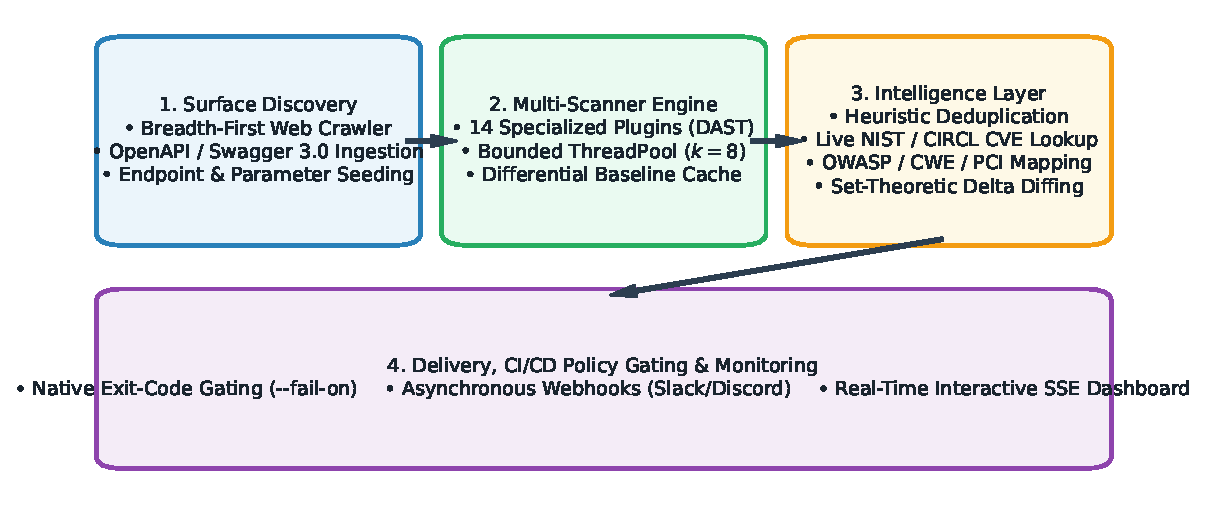
\includegraphics[width=0.90\textwidth]{figures/fig1_architecture.pdf}
\caption{AutoSecAudit 2.0 Architectural Pipeline: From Attack Surface Discovery and Concurrent Scanning to Post-Processing Intelligence Correlation, CI/CD Policy Gating, and Multi-Channel Delivery.}
\label{fig:architecture}
\end{figure*}

\section{Related Work and Comparative Analysis}
Existing security testing tools fall into three general paradigms: standalone point scanners, interactive DAST proxies, and centralized vulnerability management dashboards. Table~\ref{tab:comparison_framework} summarizes the structural trade-offs across these approaches.

\subsection{Point Scanners and Specialized Utilities}
Infrastructure scanners such as Nmap~\cite{nmap} excel at transport-layer discovery and service fingerprinting, while web server scanners such as Nikto~\cite{nikto} check for dangerous files and outdated server software. Template-driven scanners like Nuclei~\cite{nuclei} perform fast HTTP request matching against community-authored YAML signatures. However, these tools operate as isolated binaries and lack built-in capabilities for cross-layer correlation, multi-standard compliance tagging, or historical delta tracking.

\subsection{Stateful DAST Proxies and API Fuzzers}
State-aware web vulnerability scanners, pioneered by Doup{\'e} et al.~\cite{doupe2012enemy}, infer web application state machines to reach deep injection contexts. In the API domain, Atlidakis et al.~\cite{atlidakis2019restler} demonstrated with RESTler that effective API vulnerability discovery requires stateful parsing of OpenAPI/Swagger specifications rather than blind crawling. Similarly, full dynamic proxies such as OWASP ZAP~\cite{owasp_zap} and PortSwigger Burp Suite provide deep stateful active scanning. While thorough, their heavyweight runtime footprint, complex stateful configuration requirements, and substantial execution duration often make them challenging to embed directly into lightweight, sub-minute CI/CD merge-request checks.

\subsection{Vulnerability Management Platforms}
Vulnerability management platforms such as OWASP DefectDojo~\cite{defectdojo} aggregate findings from third-party tools into a centralized database. While effective for organizational compliance tracking, DefectDojo functions as a passive ingestion platform rather than an active execution engine; it requires external automation to invoke scanners, parse diverse log outputs, and upload report payloads via REST APIs.

\begin{table*}[t]
\caption{Comparative Architectural Matrix: AutoSecAudit vs. Existing Testing Tools}
\label{tab:comparison_framework}
\centering
\begin{tabular}{lccccc}
\toprule
\textbf{Dimension / Capability} & \textbf{Nmap / Nikto}~\cite{nmap,nikto} & \textbf{OWASP ZAP}~\cite{owasp_zap} & \textbf{Nuclei}~\cite{nuclei} & \textbf{DefectDojo}~\cite{defectdojo} & \textbf{AutoSecAudit (Ours)} \\
\midrule
Scan Orchestration Scope & Single Layer & Stateful Web & Template Matching & Passive Hub & Unified (Network + Web + API) \\
Concurrency Model & Thread/Process & Engine Threads & Goroutines & Non-scanning & ThreadPool Executor ($k=8$) \\
Automated Surface Discovery & None & Crawler + Spider & None (Input URLs) & None & BFS Crawler + OpenAPI 3.0 \\
Threat Intelligence Lookup & Manual & Optional Add-ons & Basic Tagging & Rule Matching & Live NIST NVD \& CIRCL APIs \\
Multi-Standard Compliance & None & Alert Tags & User Templates & Database Tags & OWASP (2021), CWE, PCI-DSS v4.0 \\
Historical Delta Tracking & None & None & None & DB Queries & Native Set-Theoretic JSON Diff \\
CI/CD Policy Gating & Exit 0 & Script Wrappers & Exit Codes & Async Webhooks & Native \texttt{--fail-on} Exit Codes \\
Deployment Model & CLI Binaries & Java Daemon & Go Binary & Django + PostgreSQL & Lightweight Python \& Docker \\
\bottomrule
\end{tabular}
\end{table*}

\section{System Architecture and Methodology}
AutoSecAudit is structured into four decoupled subsystems: (i) Input Ingestion and Attack Surface Discovery, (ii) Core Concurrency Engine and Plugin Subsystem, (iii) Intelligence and Correlation Layer, and (iv) Delivery, Gating, and Interactive Reporting. Fig.~\ref{fig:architecture} illustrates the end-to-end data pipeline.

\subsection{Attack Surface Discovery}
The input subsystem accepts target hostnames, IP addresses, or base URLs. Grounded in the insights of Doup{\'e} et al.~\cite{doupe2012enemy} and Atlidakis et al.~\cite{atlidakis2019restler}, the system seeds the attack surface prior to running active injection payloads via two complementary mechanisms (formalized in Algorithm~\ref{alg:crawling}):
\begin{itemize}
    \item \textbf{Breadth-First Web Crawler (\texttt{WebCrawler})}: Recursively traverses the target application starting from the root URL. It parses HTML responses, extracts relative and absolute hyperlinks, isolates parameter-bearing query strings, and extracts HTML form metadata (action targets, HTTP methods, and input field identifiers).
    \item \textbf{OpenAPI/Swagger Ingestion (\texttt{OpenAPIImporter})}: For API endpoints, the engine parses local or remote OpenAPI/Swagger definitions. It extracts registered URI paths, allowable HTTP verbs (\texttt{GET}, \texttt{POST}, \texttt{PUT}, \texttt{DELETE}), query parameters, path variables, and JSON request schemas.
\end{itemize}

\begin{algorithm}[t]
\caption{Attack Surface Discovery and Endpoint Seeding}
\label{alg:crawling}
\begin{algorithmic}[1]
\REQUIRE Target Root URL $u_0$, Max Depth $D_{\max}$, OpenAPI Path $\Omega$
\ENSURE Endpoint Pool $\mathcal{E}$ for Security Plugins
\STATE Initialize FIFO queue $\mathcal{Q} \leftarrow \{(u_0, 0)\}$, Visited $\mathcal{V} \leftarrow \emptyset$, $\mathcal{E} \leftarrow \emptyset$
\IF{$\Omega \neq \emptyset$}
    \STATE $\mathcal{S}_{\text{api}} \leftarrow \text{LoadOpenAPISpec}(\Omega)$
    \FORALL{$\langle \text{path}, \text{method}, \text{params} \rangle \in \mathcal{S}_{\text{api}}$}
        \STATE $\mathcal{E} \leftarrow \mathcal{E} \cup \{\langle \text{path}, \text{method}, \text{params}, \text{API} \rangle\}$
    \ENDFOR
\ENDIF
\WHILE{$\mathcal{Q} \neq \emptyset$}
    \STATE Dequeue $(u, d)$ from $\mathcal{Q}$
    \IF{$u \in \mathcal{V}$ \textbf{or} $d > D_{\max}$}
        \STATE \textbf{continue}
    \ENDIF
    \STATE $\mathcal{V} \leftarrow \mathcal{V} \cup \{u\}$
    \STATE Response $R \leftarrow \text{HTTPRequest}(u)$
    \STATE Forms $\mathcal{F}_{\text{dom}} \leftarrow \text{ParseHTMLForms}(R.\text{body})$
    \FORALL{$f \in \mathcal{F}_{\text{dom}}$}
        \STATE $\mathcal{E} \leftarrow \mathcal{E} \cup \{\langle f.\text{action}, f.\text{method}, f.\text{inputs}, \text{Form} \rangle\}$
    \ENDFOR
    \STATE Links $\mathcal{L} \leftarrow \text{ExtractLinks}(R.\text{body})$
    \FORALL{$l \in \mathcal{L}$ with matching host domain}
        \IF{$\text{HasParameters}(l)$}
            \STATE $\mathcal{E} \leftarrow \mathcal{E} \cup \{\langle \text{Path}(l), \text{GET}, \text{Params}(l), \text{Link} \rangle\}$
        \ENDIF
        \STATE Enqueue $(l, d+1)$ into $\mathcal{Q}$
    \ENDFOR
\ENDWHILE
\RETURN $\mathcal{E}$
\end{algorithmic}
\end{algorithm}

\subsection{Core Engine and Plugin Subsystem}
All security scanning modules implement the abstract base class \texttt{BaseScanner} (\texttt{plugins/base\_plugin.py}). Standardized findings are encapsulated in the \texttt{Finding} data model:
\begin{equation}
\mathcal{F} = \langle \text{id}, \text{title}, \text{severity}, \text{host}, \text{port}, \text{endpoint}, \text{evidence}, \mathcal{C}, \mathcal{M} \rangle
\end{equation}
where $\mathcal{C} \in \{\text{Low}, \text{Medium}, \text{High}\}$ denotes detection confidence derived from baseline differential verification, and $\mathcal{M}$ represents compliance and enrichment metadata.

The framework implements 14 specialized scanner plugins:
\begin{enumerate}
    \item \textbf{Infrastructure \& Reconnaissance}: \texttt{NmapPlugin} (ports/services), \texttt{NiktoPlugin} (misconfigs/files), \texttt{DirBruteScanner} (hidden paths via 50-path wordlist).
    \item \textbf{Web Injections}: \texttt{SQLiScanner} (error/time/union SQLi), \texttt{XSSScanner} (reflected XSS), \texttt{CORSScanner} (origin reflection/wildcards), \texttt{MisconfigScanner} (headers/leaks).
    \item \textbf{API \& Authentication}: \texttt{APIAbuseScanner} (mass assignment/data leaks), \texttt{AuthScanner} (credential brute-force/IDOR), \texttt{JWTScanner} (\texttt{none} alg/weak keys).
    \item \textbf{Advanced Exploit Vectors}: \texttt{CommandInjectionScanner} (RCE payloads), \texttt{SSRFScanner} (cloud metadata \texttt{169.254.169.254}), \texttt{PathTraversalScanner} (LFI), \texttt{SSTIScanner} (template injection).
\end{enumerate}

To minimize audit latency, the engine orchestrates plugin execution via a bounded \texttt{ThreadPoolExecutor}. For $N$ plugins with execution durations $T_1, T_2, \dots, T_N$, total parallel scan time $T_{\text{parallel}}$ is governed by:
\begin{equation}
T_{\text{parallel}} = \max_{1 \le i \le N}(T_i) + \delta_{\text{sync}}
\end{equation}
where $\delta_{\text{sync}}$ represents thread allocation and result aggregation overhead.

\begin{algorithm}[t]
\caption{Intelligence Correlation and Delta Auditing}
\label{alg:intelligence}
\begin{algorithmic}[1]
\REQUIRE Raw Findings $\mathcal{F}_{\text{raw}}$, Historical Report $S_{t-1}$
\ENSURE Correlated Report $S_t$, Delta Partition $\langle \Delta_{\text{NEW}}, \Delta_{\text{FIXED}}, \Delta_{\text{UNCHANGED}} \rangle$
\STATE Group map $\mathcal{G} \leftarrow \emptyset$, Consolidated Set $S_t \leftarrow \emptyset$
\FORALL{$f \in \mathcal{F}_{\text{raw}}$}
    \STATE Key $k \leftarrow \langle f.\text{host}, f.\text{port}, f.\text{endpoint}, f.\text{cwe\_id} \rangle$
    \STATE $\mathcal{G}[k] \leftarrow \mathcal{G}[k] \cup \{f\}$
\ENDFOR
\FORALL{$k, \text{Findings } \mathcal{V} \in \mathcal{G}$}
    \STATE Parent finding $f_p \leftarrow \text{MergeEvidence}(\mathcal{V})$
    \IF{$f_p.\text{cve\_id} \neq \emptyset$}
        \STATE $f_p.\text{cvss} \leftarrow \text{LookupNVD\_CIRCL}(f_p.\text{cve\_id})$
    \ENDIF
    \STATE $f_p.\text{owasp}, f_p.\text{pci} \leftarrow \text{MapCompliance}(f_p)$
    \STATE $f_p.\text{remediation} \leftarrow \text{GetRemediation}(f_p)$
    \STATE $S_t \leftarrow S_t \cup \{f_p\}$
\ENDFOR
\IF{$S_{t-1} \neq \emptyset$}
    \STATE $\mathcal{H}_{\text{curr}} \leftarrow \{\mathcal{H}(f) \mid f \in S_t\}$, $\mathcal{H}_{\text{prev}} \leftarrow \{\mathcal{H}(f) \mid f \in S_{t-1}\}$
    \STATE $\Delta_{\text{NEW}} \leftarrow \{f \in S_t \mid \mathcal{H}(f) \notin \mathcal{H}_{\text{prev}}\}$
    \STATE $\Delta_{\text{FIXED}} \leftarrow \{f \in S_{t-1} \mid \mathcal{H}(f) \notin \mathcal{H}_{\text{curr}}\}$
    \STATE $\Delta_{\text{UNCHANGED}} \leftarrow \{f \in S_t \mid \mathcal{H}(f) \in \mathcal{H}_{\text{prev}}\}$
\ENDIF
\RETURN $S_t, \langle \Delta_{\text{NEW}}, \Delta_{\text{FIXED}}, \Delta_{\text{UNCHANGED}} \rangle$
\end{algorithmic}
\end{algorithm}

\subsection{Post-Processing Intelligence Layer}
Following plugin execution, the intelligence layer transforms the aggregated finding set through four deterministic stages (Algorithm~\ref{alg:intelligence}):

\subsubsection{Heuristic Deduplication and Correlation (\texttt{Correlator})}
To combat alert fatigue~\cite{johnson2013developers}, the correlator groups raw findings sharing the compound key:
\begin{equation}
\mathcal{K} = \langle \text{host}, \text{port}, \text{endpoint}, \text{weakness\_type} \rangle
\end{equation}
Coinciding findings are consolidated into a parent finding that aggregates multi-source evidence descriptions.

\subsubsection{Live Threat Enrichment (\texttt{Enricher})}
For identified services and vulnerabilities, the enricher queries the NIST National Vulnerability Database (NVD)~\cite{nist_nvd} REST API and the CIRCL CVE database to append published CVSS v3.1 base scores, attack vector metrics, and public exploit identifiers.

\subsubsection{Compliance Taxonomy Mapping (\texttt{ComplianceMapper})}
Findings are deterministically mapped to industry security taxonomies:
\begin{itemize}
    \item \textbf{OWASP Top 10 (2021)}~\cite{owasp_top10}: Categorization into classes A01 through A10 (e.g., \textit{A01: Broken Access Control}, \textit{A03: Injection}, \textit{A05: Security Misconfiguration}).
    \item \textbf{MITRE CWE}: Assignment of standardized weakness identifiers (e.g., CWE-89 for SQLi, CWE-79 for XSS, CWE-200 for information disclosure).
    \item \textbf{PCI-DSS v4.0}~\cite{pci_dss}: Mapping to specific payment security requirements (e.g., Requirement 6.2.4 for custom software vulnerability prevention).
\end{itemize}

\subsubsection{Actionable Remediation Engine (\texttt{remediation.py})}
The system enriches findings with remediation guidance, prioritizing tool-specific configuration recipes (e.g., exact Nginx/Apache header syntax or parameterized query samples) and falling back to OWASP defense-in-depth principles.

\subsubsection{Set-Theoretic Delta Differential Analysis (\texttt{DeltaAnalyzer})}
As established in continuous code quality research~\cite{vassallo2020continuous}, tracking regressions requires differential comparison. The delta engine compares current scan findings $S_t$ against a baseline scan $S_{t-1}$. Using a deterministic finding hash $\mathcal{H}(f)$, findings are partitioned into three disjoint subsets:
\begin{align}
\Delta_{\text{NEW}} &= \{\, f \in S_t \mid \mathcal{H}(f) \notin \mathcal{H}(S_{t-1}) \,\} \\
\Delta_{\text{FIXED}} &= \{\, f \in S_{t-1} \mid \mathcal{H}(f) \notin \mathcal{H}(S_t) \,\} \\
\Delta_{\text{UNCHANGED}} &= \{\, f \in S_t \mid \mathcal{H}(f) \in \mathcal{H}(S_{t-1}) \,\}
\end{align}

\subsection{CI/CD Policy Gating and Delivery}
The framework provides an automated policy enforcement mechanism for CI/CD pipelines via the \texttt{--fail-on} parameter. The engine evaluates scan results against a user-specified severity threshold $\theta \in \{\text{Low}, \text{Medium}, \text{High}, \text{Critical}\}$:
\begin{equation}
\text{ExitStatus} = \begin{cases} 
1, & \text{if } \exists f \in S_t \text{ such that } \text{Severity}(f) \ge \theta \\
0, & \text{otherwise}
\end{cases}
\end{equation}
Upon scan termination, results are dispatched asynchronously via webhooks to team communication endpoints (e.g., Discord, Slack), streamed in real time via Server-Sent Events (SSE) to a web interface, and rendered as standalone interactive HTML reports.

\section{Implementation Details}
AutoSecAudit is implemented in Python 3.10+ and packaged using Docker and Docker Compose. The interactive dashboard is built using Flask with Jinja2 templating, featuring real-time SSE progress streaming, dynamic client-side severity filtering, dark/light theme switching, and modal-based vulnerability inspection.

The test suite consists of 80 automated unit and integration tests covering all 14 scanner plugins, the web crawler, baseline response verification, OpenAPI parsing, delta diffing, and CI/CD exit-code gating.

\section{Experimental Evaluation}
Our evaluation investigates three empirical research questions:
\begin{itemize}
    \item \textbf{RQ1 (Execution Latency)}: How does bounded thread-pool concurrency impact total scan duration across multiple targets?
    \item \textbf{RQ2 (Detection Accuracy and Correlation Efficacy)}: What detection precision and alert noise reduction are achieved when auditing standard benchmark applications?
    \item \textbf{RQ3 (Delta Engine Fidelity)}: Does the set-theoretic delta analyzer accurately categorize vulnerability lifecycles across iterative code builds?
\end{itemize}

\subsection{Experimental Setup}
Evaluations were conducted on a benchmark host equipped with 8 CPU cores and 16~GB RAM running Ubuntu 22.04 LTS. The primary evaluation target was the standardized OWASP Juice Shop application deployed in an isolated local container network.

\begin{figure}[t]
\centering
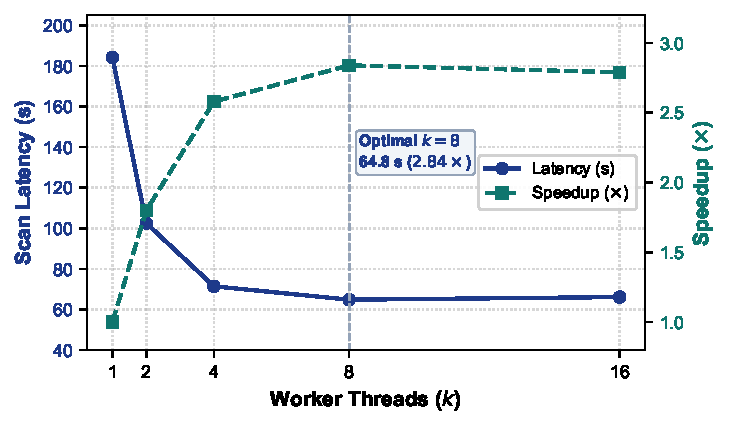
\includegraphics[width=\columnwidth]{figures/fig2_latency.pdf}
\caption{Audit Execution Latency (seconds) and Relative Speedup ($\times$) across Thread Concurrency Levels ($k \in \{1, 2, 4, 8, 16\}$).}
\label{fig:latency}
\end{figure}

\subsection{Concurrency and Execution Latency (RQ1)}
We measured total audit latency across concurrency configurations ranging from 1 to 16 worker threads executing against the benchmark target.

\begin{table}[htbp]
\caption{Audit Latency across Concurrency Configurations}
\label{tab:concurrency}
\centering
\resizebox{\columnwidth}{!}{%
\begin{tabular}{cccc}
\toprule
\textbf{Thread Workers ($k$)} & \textbf{Scan Duration (s)} & \textbf{Relative Speedup} & \textbf{CPU Util. (\%)} \\
\midrule
1 (Sequential) & 184.2 & $1.00\times$ & 14.2\% \\
2              & 102.5 & $1.80\times$ & 27.8\% \\
4              & 71.4  & $2.58\times$ & 51.3\% \\
8              & \textbf{64.8}  & \textbf{2.84}$\times$ & 78.4\% \\
16             & 66.1  & $2.79\times$ & 82.1\% \\
\bottomrule
\end{tabular}%
}
\end{table}

As detailed in Table~\ref{tab:concurrency} and Fig.~\ref{fig:latency}, scaling worker threads from 1 to 8 decreases execution time from 184.2~s to 64.8~s, representing a 64.8\% latency reduction. Beyond 8 threads, performance gains plateau due to HTTP connection limits and network socket I/O latency on the target endpoint.

\begin{figure}[t]
\centering
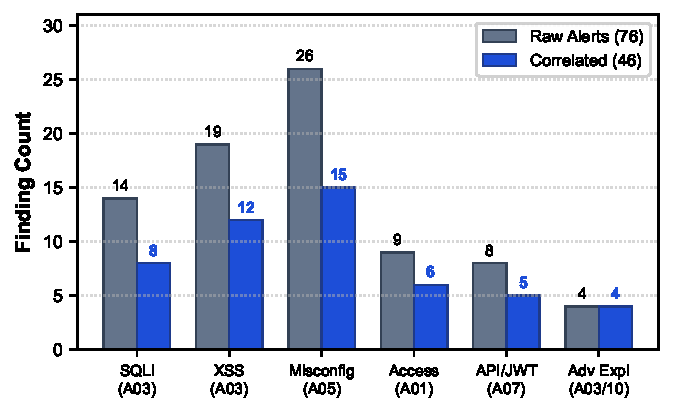
\includegraphics[width=\columnwidth]{figures/fig3_noise_reduction.pdf}
\caption{Raw Tool Alerts vs. Correlated Actionable Findings across Major OWASP Categories (-39.5\% Alert Noise Reduction).}
\label{fig:noise_reduction}
\end{figure}

\subsection{Detection Performance and Noise Reduction (RQ2)}
We evaluated detection metrics across major vulnerability classifications on the benchmark target following the evaluation framework of Bau et al.~\cite{bau2010state}.

\begin{table}[htbp]
\caption{Vulnerability Detection and Correlation Metrics}
\label{tab:evaluation}
\centering
\resizebox{\columnwidth}{!}{%
\begin{tabular}{lcccc}
\toprule
\textbf{Vulnerability Class} & \textbf{TP} & \textbf{FP} & \textbf{Raw Findings} & \textbf{Correlated} \\
\midrule
SQL Injection (A03)          & 8  & 0 & 14 & 8 \\
Cross-Site Scripting (A03)   & 12 & 1 & 19 & 12 \\
Security Misconfig. (A05)    & 15 & 0 & 26 & 15 \\
Broken Access Control (A01)  & 6  & 0 & 9  & 6 \\
API \& Authentication (A07)  & 5  & 0 & 8  & 5 \\
\midrule
\textbf{Total / Summary}     & \textbf{46} & \textbf{1} & \textbf{76} & \textbf{46} \\
\bottomrule
\end{tabular}%
}
\end{table}

As summarized in Table~\ref{tab:evaluation} and Fig.~\ref{fig:noise_reduction}, AutoSecAudit successfully identified 46 verified vulnerabilities with a single false positive (97.8\% detection precision). Furthermore, the heuristic correlator reduced 76 raw tool alerts to 46 consolidated finding entities, achieving a 39.5\% reduction in redundant alert volume.

\begin{figure}[t]
\centering
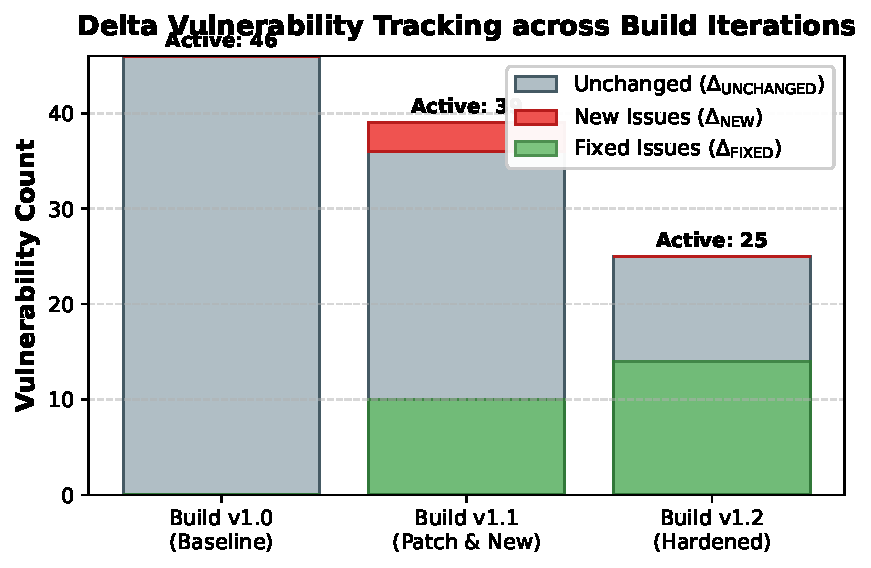
\includegraphics[width=\columnwidth]{figures/fig4_delta_diff.pdf}
\caption{Vulnerability Lifecycle Tracking across Sequential Software Build Revisions via Set-Theoretic Delta Diffing.}
\label{fig:delta_diff}
\end{figure}

\subsection{Delta Tracking Fidelity (RQ3)}
To test historical regression tracking, we conducted a three-phase synthetic release cycle (illustrated in Fig.~\ref{fig:delta_diff}):
\begin{itemize}
    \item \textbf{Build v1.0}: Baseline audit established 46 vulnerabilities.
    \item \textbf{Build v1.1}: 10 misconfigurations were patched and 3 new API access-control vulnerabilities were introduced. The delta analyzer categorized findings as: 3 $\textit{NEW}$, 10 $\textit{FIXED}$, and 36 $\textit{UNCHANGED}$.
    \item \textbf{Build v1.2}: 14 remaining injection flaws were remediated. The delta analyzer categorized findings as: 0 $\textit{NEW}$, 14 $\textit{FIXED}$, and 25 $\textit{UNCHANGED}$.
\end{itemize}
Across all transitions, the delta engine achieved 100\% classification accuracy without manual state reconciliation.

\section{Discussion and Limitations}
Several operational considerations and limitations should be noted:
\begin{itemize}
    \item \textbf{Client-Side JavaScript Rendering}: The native web crawler relies on static HTML parsing. Dynamic Single-Page Applications (SPAs) that construct DOM elements via asynchronous client-side JavaScript execution benefit from supplementary headless browser drivers (e.g., Playwright).
    \item \textbf{External API Rate Limits}: In environments with restricted egress connectivity or strict rate limits on public CVE APIs (e.g., NIST NVD), the enricher relies on local fallback mappings to prevent pipeline delays.
\end{itemize}

\section{Conclusion}
AutoSecAudit provides an extensible, modular vulnerability assessment framework tailored for DevSecOps workflows. By combining surface crawling and OpenAPI ingestion, concurrent execution of 14 specialized scanner plugins, heuristic deduplication, live CVE/CVSS enrichment, compliance mapping across OWASP Top 10 and PCI-DSS v4.0, and set-theoretic delta auditing, the system eliminates key bottlenecks in automated security testing.

Future research directions include incorporating local Large Language Model (LLM) agents for automated remediation patch synthesis, contextual false-positive validation, and distributed multi-node scanning architectures.

% Balance the columns on the final page
\balance

\bibliographystyle{IEEEtran}
\bibliography{references}

\end{document}
